\section{Architecture}\label{{sec:architecture}}
Although this paper goals aim solely on the scheduler and introducing the new load balancing strategy,
the architecture keeps in mind the future work outlined in section \ref{sec:future-work}.
Therefore the system's architecture is based on the idea of cooperating microservices,
where each service has control over a specific part of the infrastructure. 

Microservice architecture is a software design architectural style 
that structures an application as a collection of loosely coupled services that are organized around the system's business capabilities\cite{namiot2014micro} 
and are independently deployable with enabled continuous delivery\cite{balalaie2016microservices}.
Microservice architectural design also helps the system's better horizontal scalability
by using multiple instances of one microservice 
and the orchestration module.

\subsection{Architecture scheme}\label{subsec:architecture-scheme}
Scheme \ref{fig:scheduling-core-arch} visualizes only system's core architecture. 
However,
the whole design keeps in mind future infrastructure development proposed in section \ref{sec:future-work}.
The implementation itself was developed accordingly 
and used technologies and techniques are described in the following sections.

\begin{figure}[ht]
    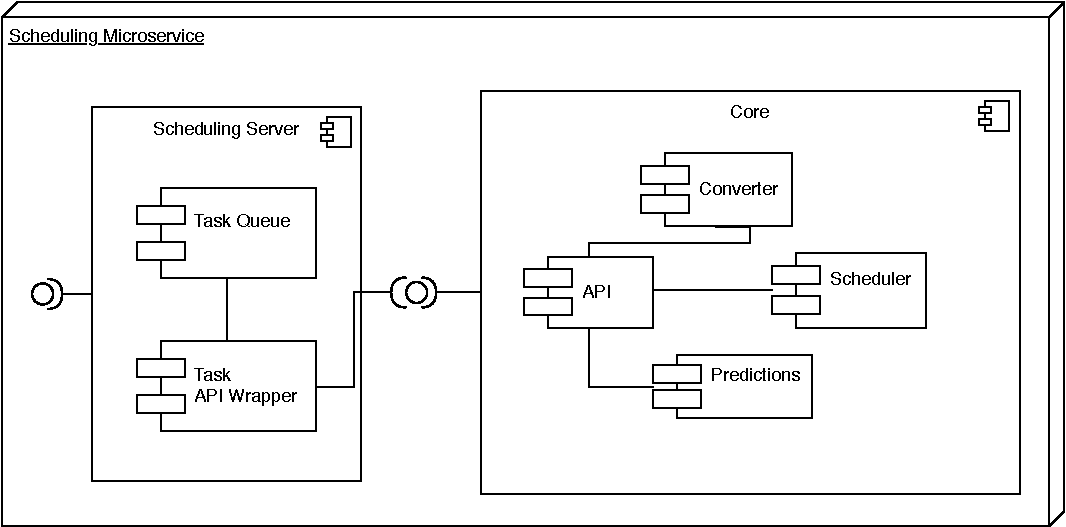
\includegraphics[width=\textwidth]{i_scheduler.pdf} 
    \centering
    \caption{Microservice architecture with scheduling core}
    \label{fig:scheduling-core-arch}
\end{figure}

Core component, 
which is responsible for scheduling and load balancing,
is composed of API, converter, predictions, and scheduler module.
\begin{itemize}
    \item \textit{API module} implements common core interface \inlinecode{OlbCoreApi} 
    and is responsible for scheduling requests handling.
    Actual implementation of API interface is class \inlinecode{OlbCoreApiImpl}.
    \item \textit{Converter module} is used to convert received input data into scheduler's inner data representation and then back to common data transfer objects. 
    This converter is implemented as a class \inlinecode{InputToDomainConverter}.
    \item \textit{Scheduler module} contains constraints, evaluator and scheduling system based on OptaPlanner solution
    (described in section \ref{sec:load-balancing-optaplanner}).
    Scheduler module consist of multiple packages, 
    \inlinecode{constraints} - containing all constrains for scheduling algorithm,
    \inlinecode{domain} with defined scheduling domain for OptaPlanner,
    \inlinecode{evaluation} which includes evaluator calculating planning score
    and \inlinecode{solver} package with factory initializing OptaPlanner scheduling core.
\end{itemize}

Scheduling server provides HTTP API access to the core
and serves as the microservice base.
The server module is based on Ktor framework (described in section \ref{subsec:framework})
that runs under the hood and provides HTTP functionality.,
The server API uses binary serialization and accepts data transfer objects used in the solutions.
This serialization approach was chosen because of the number of interfaces and loosely coupled data objects,
that are being used in the application.

\subsubsection{Simulations architecture}\label{subsec:simulations-architecture}
Simulations module (project module \inlinecode{simulations}) is designed as another microservice to simulate future load balancing system's behavior.
Following figure \ref{fig:simulations-arch} shows the architecture of the module.  

\begin{figure}[ht]
    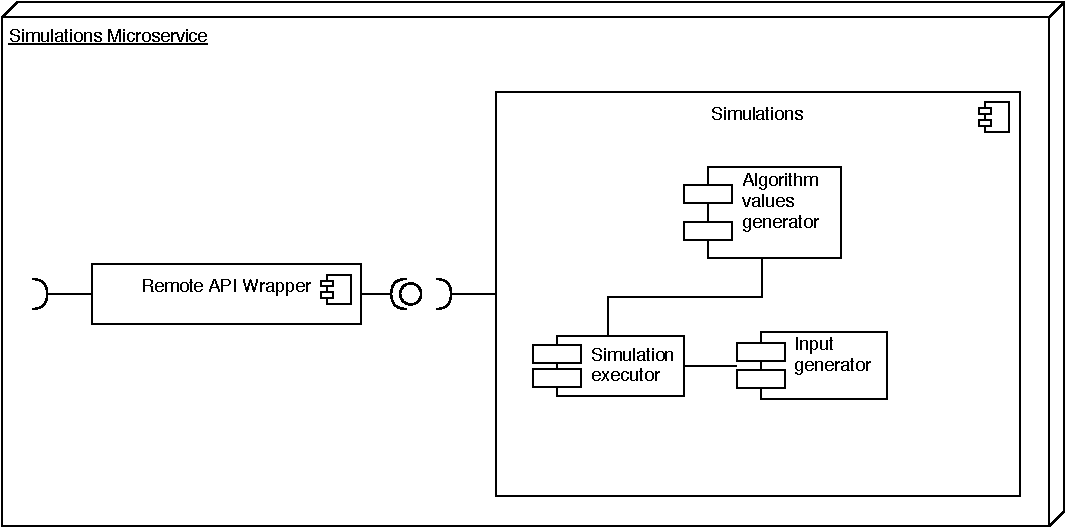
\includegraphics[width=\textwidth]{i_simulations.pdf}
    \centering
    \caption{Simulations module scheme}
    \label{fig:simulations-arch}
\end{figure}

Input data are generated by the input generator module,
which can be found, for example in \inlinecode{DomainBuilder} class.
Algorithm values are parsed from the file in class \inlinecode{DataParser} 
and the corresponding model is created on top of them in \inlinecode{JobWithHistoryFactory}.

Remote API wrapper is used to create a connection between remote microservice, with scheduling API, and simulation.
For the simulation module,
the connection seems to be synchronous.
It is because there is a blocking queue used to store and answer the calls between these two microservices.
Thanks to this solution,
simulations can be run in a microservices mode as well as locally without any additional effort needed.
Remote scheduling solution is implemented in the project module \inlinecode{remote-scheduler}.
Local simulations can be found for example in \inlinecode{OnePlanningRoundMain} or \inlinecode{ExecutionConfiguration} classes.